\documentclass[]{article}
\usepackage[utf8]{inputenc}
\usepackage{polski}
\usepackage{listings}
\usepackage[usenames,dvipsnames]{xcolor}
\usepackage{geometry}
\usepackage{subcaption}
\usepackage{graphicx}
\usepackage{amsmath}
\usepackage{amssymb}
\usepackage{enumerate}
\DeclareGraphicsExtensions{.png}
\graphicspath{ {./} }
\geometry{
	a4paper,
	left=25mm,
	right = 25mm,
	top=25mm,
}
%%\hyphenchar\font=-1

\title{
	Sprawozdanie \\
	\large 
	Obliczenia naukowe - lista 3}
\author{Kamil Król}
\date{244949}


\begin{document}
	
	\maketitle
	
	\section*{Zadanie 1}
	Celem tego zadania było powtórzenie zadania 5 z listy 1, ale ze zmianą danych i 
	
	\section*{Zadanie 2}
	
	Celem zadania 

	\section*{Zadanie 3} 
	
	Celem zadania 
	
	\section*{Zadanie 4}

	Celem zadania było wyznaczenie pierwiastków równania $\sin{x}-(\frac{1}{2}x)^2 = 0$ używając wcześniej zaimplementowanych metod:
	\begin{enumerate}[(a)]
		\item metody bisekcji (z przedziałem początkowym $[1.5, 2.0]$),
		\item metody Newtona (z przybliżeniem początkowym $x_0 = 1.5$),  
		\item metody siecznych (z przybliżeniami początkowymi $x_0 = 1.0$ i $x_1 = 2.0$).
	\end{enumerate}
	Dla wszystkich metod dokładności były wspólne tj. $\delta = \epsilon = \frac{1}{2}10^{-5}$. Za maksymalną liczbę iteracji przyjąłem 40. Zacząłem od obliczenia pochodnej funkcji $f$, $f'(x) = \cos{x} - \frac{1}{2}x$ potrzebnej w metodzie Newtona. Wyniki działania programów znajdują się w tabeli poniżej.
	
	\begin{table}[h!]
		\centering
		\label{tab:table1}
		\begin{tabular}{|c|c|c|c|}
			\hline
			metoda & wartość pierwiastka - $r$ & wartość funkcji w punkcie $r$ - $f(r)$ & liczba iteracji \\ \hline
			metoda bisekcji & 1.9337539672851562 & -2.7027680138402843e-7 & 16 \\ \hline
			metoda Newtona & 1.933753779789742 & -2.2423316314856834e-8 & 4 \\ \hline
			metoda siecznych & 1.933753644474301 & 1.564525129449379e-7 & 4 \\ \hline
		\end{tabular}
	\end{table}
	
	Widać, że różnica w ilości wykonanych iteracji między metodą bisekcji a dwoma pozostałymi jest znaczna. Metoda bisekcji okazała się najwolniejsza. Metody Newtona i siecznych okazały się w tym przypadku porównywalne jeśli chodzi o ilość iteracji potrzebną do osiągnięcia zadanej dokładności. Wyniki eksperymentu mają odzwierciedlenie w teorii. Współczynnik zbieżności dla metody siecznych wynosi $1$ (zbieżność liniowa), dla metody Newtona $2$ (zbieżność kwadratowa), a dla metody siecznych $\approx1.62$.
	
	\clearpage
	
	\section*{Zadanie 5}
	Celem zadania było użycie metody bisekcji do znalezienia, wartości zmiennej $x$, dla której przecinają się wykresy funkcji $y=3x$ oraz $y=e^x$. Zadane dokładności wynosiły $\delta = \epsilon = 10^{-4}$. Zadanie można sprowadzić do problemu rozwiązania równania $e^x - 3x = 0$ lub równoważnie znalezienia miejsc zerowych funkcji $f(x) = e^x - 3x$. Pierwszą rzeczą jaką należało wykonać to dobrać przedział lub przedziały początkowe. Wiemy, że metoda bisekcji wymaga takiego przedziału, że wartości funkcji w jego końcach mają różny znak. W celu wyznaczenia przedziałów początkowych posłużyłem się poniższymi wykresami.
	
	\begin{figure}[!htbp]
		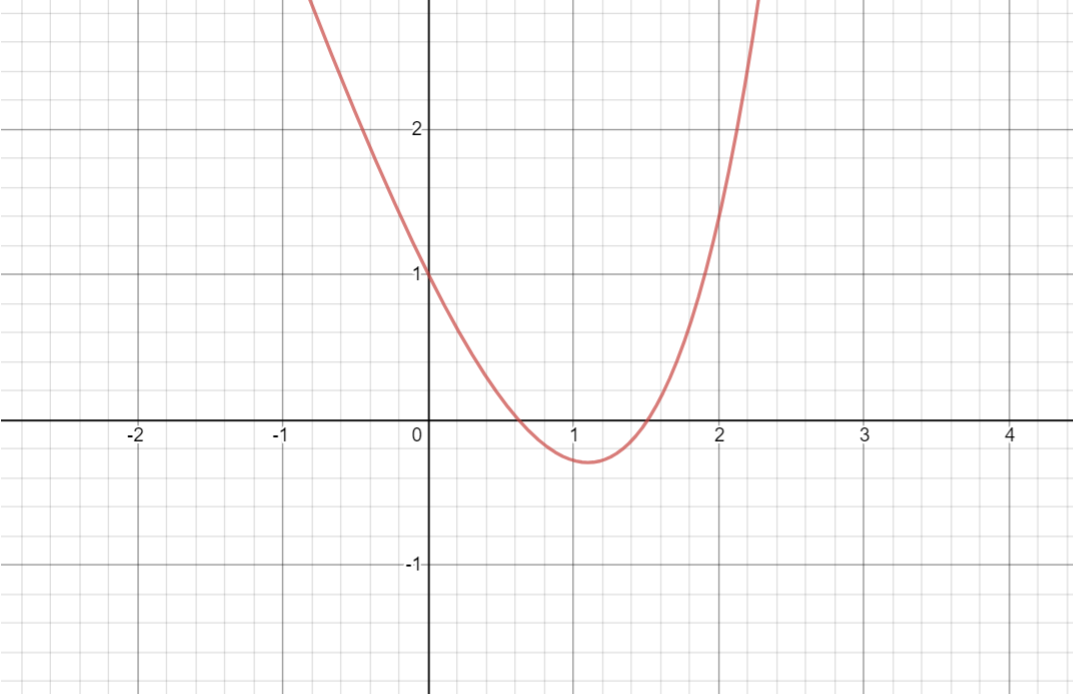
\includegraphics[width=\textwidth]{task5plot}
		\centering
		\caption{Wykres funkcji $f(x) = e^x - 3x$}
	\end{figure}
	
%	\begin{figure}[!htbp]
%		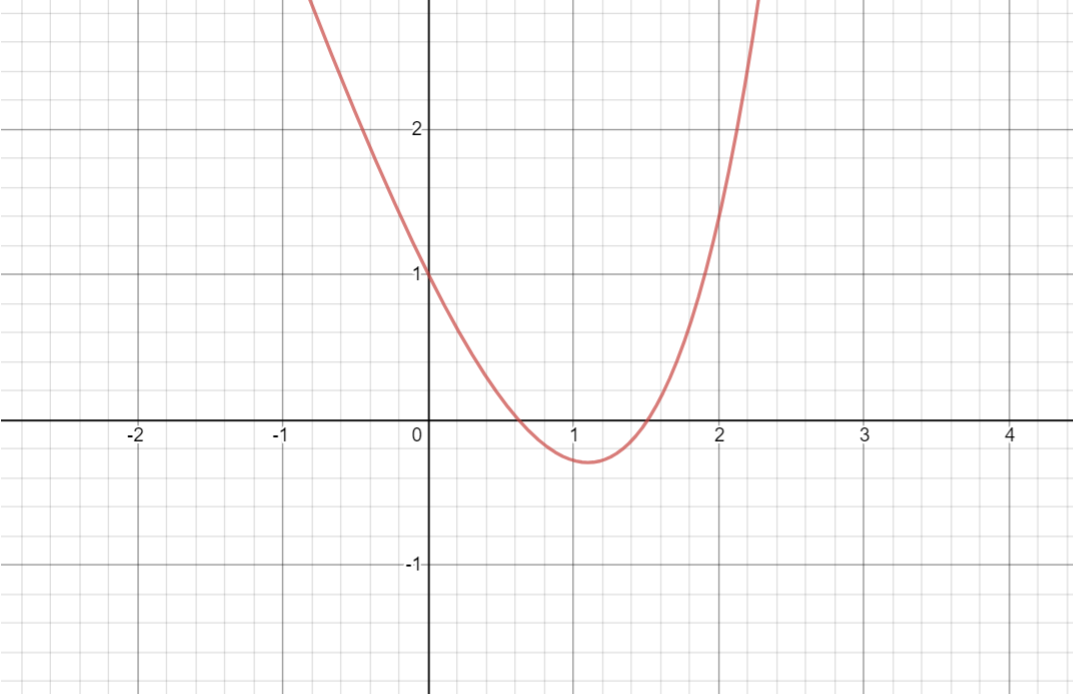
\includegraphics[height=0.38\textheight]{task5plot}
%		\centering
%		\caption{Wykres funkcji $f(x) = e^x - 3x$}
%	\end{figure}
%	\begin{figure}[!htbp]
%		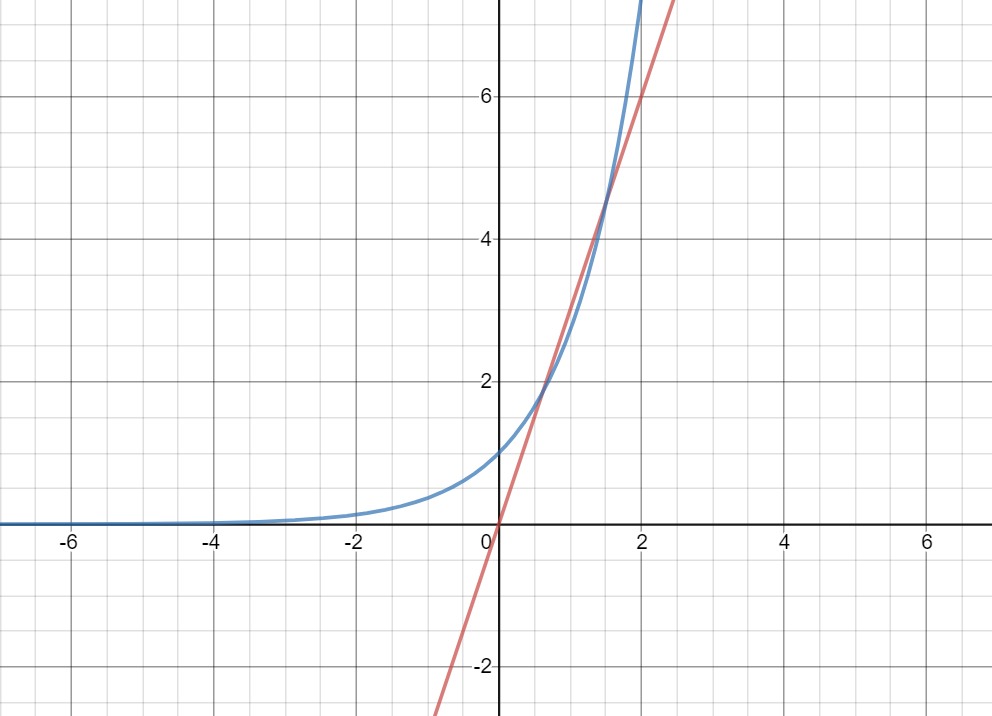
\includegraphics[height=0.36\textheight]{3xexplot}
%		\centering
%		\caption{Wykresy funkcji $e^x$ i $3x$}
%	\end{figure}

	Patrząc na wykresy wybrałem przedziały [0,1] oraz [1,2]. Oba z nich spełniają wymagania metody bisekcji. Znalezione pierwiastki to $x_1=0.619140625$ oraz $x_2=1.5120849609375$ co pokrywa się z tym co sugeruje wykres.
	
	
	\begin{table}[!h]
		\centering
		\label{tab:table1}
		\begin{tabular}{c|c|c}
			
			 & $x_1$ & $x_2$ \\ \hline
			Wartość pierwiastka $r$ &  0.619140625 & 1.5120849609375 \\ 
			Wartość funkcji $f(r)$ & -9.066320343276146e-5 & -7.618578602741621e-5  \\ 
			Liczba iteracji & 9 & 13 \\
			Przedział & [0,1] & [1,2] \\
		\end{tabular}
	\end{table}

	Widać, że oba pierwiastki występują dość blisko siebie oraz fakt, że znacznym ułatwieniem w znaleznieniu przedziałów początkowych była znajomość przebiegu funkcji $f$. Na wykresie od razu widać było, że powinniśmy się spodziewać dokładnie dwóch miejsc zerowych oraz gdzie się ich spodziewać. Bez pomocy jaką była znajomość przebiegu funkcji $f$ nie wiedzielibyśmy nawet ilu miejsc zerowych powinniśmy się spodziewać. Innym wnioskiem jest fakt, że znalezione miejsce zerowe zależy od wybranego przedziału początkowego. Ogólniejszym wnioskiem jest to, że bez dobrej znajomości przebiegu funkcji metoda bisekcji może być problematyczna do zastosowania. 

	\clearpage

	W tabeli poniżej znajdują się wyniki eksperymentu drugiego, który polegał na wykonaniu 40 iteracji tego samego wyrażenia rekurencyjnego w arytmetyce Float32 oraz Float64 dla danych $p_0 = 0.01$ i $r = 3$, a później porównaniu otrzymanych wyników.

		\begin{table}[!h]
		\centering
		\label{tab:table1}
		\begin{tabular}{|c|c|c|c|}
			\hline
			numer iteracji & Float32 & Float64 \\
			\hline
			1 & 0.0397      	    &  0.0397 \\ \hline
			2 & 0.15407173  		& 0.15407173000000002 \\ \hline
			3 & 0.5450726   		& 0.5450726260444213 \\ \hline
			4 & 1.2889781   		& 1.2889780011888006 \\ \hline
			5 & 0.1715188   		& 0.17151914210917552 \\ \hline
			6 & 0.5978191   		& 0.5978201201070994 \\ \hline
			7 & 1.3191134   		& 1.3191137924137974 \\ \hline
			8 & 0.056273222 		& 0.056271577646256565 \\ \hline
			9 & 0.21559286  		& 0.21558683923263022 \\ \hline
			10 & 0.7229306  		& 0.722914301179573 \\ \hline
			11 & 1.3238364  		& 1.3238419441684408 \\ \hline
			12 & 0.037716985		& 0.03769529725473175 \\ \hline
			13 & 0.14660022 		& 0.14651838271355924 \\ \hline
			14 & 0.521926   		& 0.521670621435246 \\ \hline
			15 & 1.2704837  		& 1.2702617739350768 \\ \hline
			16 & 0.2395482  		& 0.24035217277824272 \\ \hline
			17 & 0.7860428  		& 0.7881011902353041 \\ \hline
			18 & 1.2905813  		& 1.2890943027903075 \\ \hline
			19 & 0.16552472 		& 0.17108484670194324 \\ \hline
			20 & 0.5799036  		& 0.5965293124946907 \\ \hline
			21 & 1.3107498  		& 1.3185755879825978 \\ \hline
			22 & 0.088804245		& 0.058377608259430724 \\ \hline
			23 & 0.3315584  		& 0.22328659759944824 \\ \hline
			24 & 0.9964407  		& 0.7435756763951792 \\ \hline
			25 & 1.0070806  		& 1.315588346001072 \\ \hline
			26 & 0.9856885  		& 0.07003529560277899 \\ \hline
			27 & 1.0280086  		& 0.26542635452061003 \\ \hline
			28 & 0.9416294  		& 0.8503519690601384 \\ \hline
			29 & 1.1065198  		& 1.2321124623871897 \\ \hline
			30 & 0.7529209  		& 0.37414648963928676 \\ \hline
			31 & 1.3110139  		& 1.0766291714289444 \\ \hline
			32 & 0.0877831  		& 0.8291255674004515 \\ \hline
			33 & 0.3280148  		& 1.2541546500504441 \\ \hline
			34 & 0.9892781  		& 0.29790694147232066 \\ \hline
			35 & 1.021099   		& 0.9253821285571046 \\ \hline
			36 & 0.95646656 		& 1.1325322626697856 \\ \hline
			37 & 1.0813814  		& 0.6822410727153098 \\ \hline
			38 & 0.81736827 		& 1.3326056469620293 \\ \hline
			39 & 1.2652004  		& 0.0029091569028512065 \\ \hline
			40 & 0.25860548 		& 0.011611238029748606 \\ \hline
		\end{tabular}
	\end{table}

	Z pierwszej tabeli widać, że zaburzenie wartości w 10 iteracji zmienia całkowicie wyniki w dalszych iteracjach. Od tego miejsca nie widać żadnej zależności między wynikami. Widać zatem, że w przypadku równania rekurencyjnego małe zaburzenie danych całkowicie zmieniło następne wyniki. Kolejna tabela pokazuje doświadczenie gdzie żadne zaburzenie nie zostało wprowadzone, jedyna różnica to arytmetyka w jakiej były wykonywane obliczenia. Widać, że na początku wartości są podobne, ale później tak jak w poprzednim eksperymencie zaczynają od siebie odbiegać dając na końcu zupełnie różne wyniki. Oba eksperymenty ukazują jak drobne błędy np. te związane z dokładnością przechowywanych danych mogą się kumulować i wpływać na wyniki. 
	Jest to zjawisko chaosu w układach sprzężeń zwrotnych. Czym są układy sprzężeń zwrotnych? Są to układy gdzie dane wyjściowe jednego procesu są danymi wejściowymi dla kolejnego kroku obliczeń. Wnioskiem z zadania jest to, że to równanie rekurencyjne jest niestabilne. Ponadto widać, że zjawisko chaosu jest trudne lub wręcz niemożliwe do wyeliminowania - dokładność obliczeń możemy ulepszyć poprzez zwiększanie precyzji arytmetyki, ale dla każdej arytmetyki pojawi się moment, w którym obliczenia stracą dokładność. 
	
	\section*{Zadanie 6}
	
	Celem zadania było sprawdzenie zachowania pewnego równania rekurencyjnego poprzez wykonanie 40 iteracji dla podanych w treści zadania zestawów danych. Równanie:
	$$x_{n+1} := x^2_n + c, \ \textrm{dla} \ n = 0,1,\dots$$
	
	Wyniki znajdują się w tabelach na końcu paragrafu.
	
	

	Obserwując wyniki dla c = -2 widać, że dla $x_0 = 1$ oraz dla $x_0 = 2$ rekurencja okazała się stabilna. Inna rzecz jaką można zauważyć, to fakt, że dla wartości nieznacznie odchylonej od 2.0 tzn. $x_0 = 1.99999999999999$ wyniki są zupełnie różne niż dla $x_0 = 2$. Widać zatem bardzo dużą czułość na warunki początkowe. Obserwując wyniki dla $c = -1$ widać, że otrzymane ciągi dla $x_0 = 1$ jak i $x_0 = -1$ są identyczne. Wynika to z podnoszenia tej wartości do kwadratu. Ostatnie dwie kolumny pokazują sytuację gdzie oba ciągi po jakimś czasie się stabilizują. Zarówno dla $x_0 = 0.25$ jak i $x_0 = 0.75$ otrzymujemy naprzemienne ciągi -1 i 1. Poniżej iteracje graficzne.
	

\begin{figure}[!htbp]
	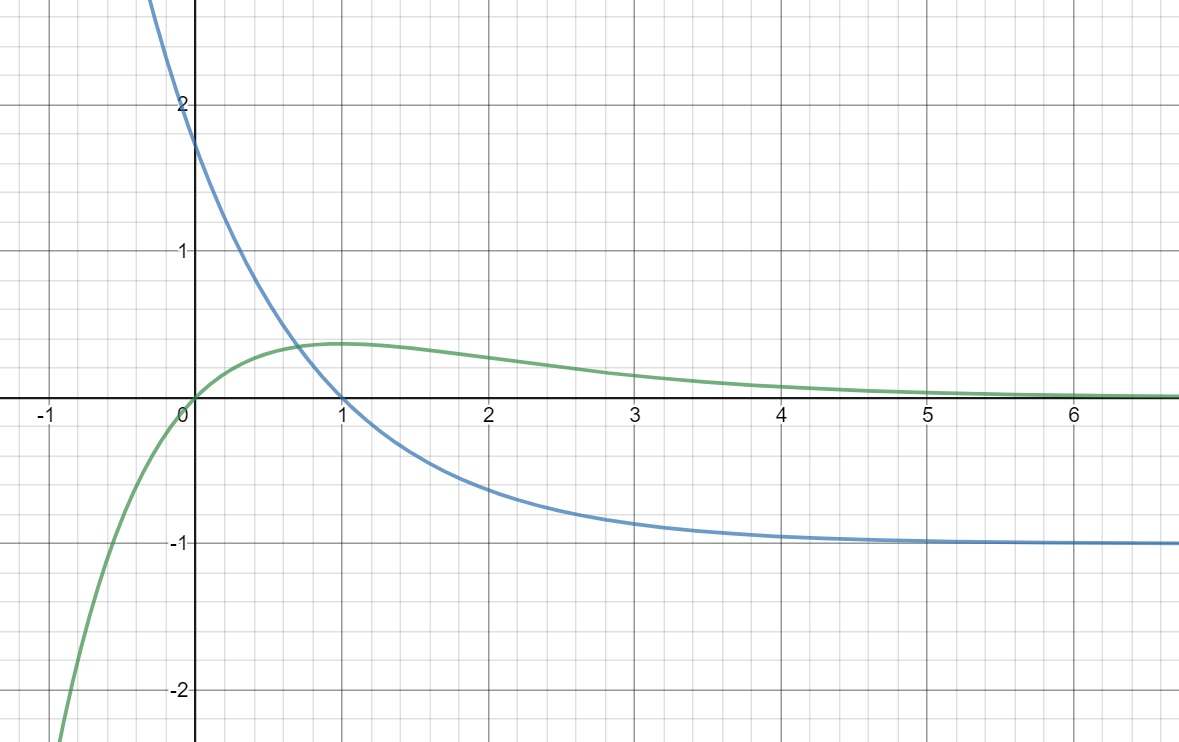
\includegraphics[scale=1]{e1-x-1andxe-x.png}
	\centering
	\caption{$c = -2$, $x_0 = 1$}
\end{figure}
\clearpage
\begin{figure}[!htbp]
	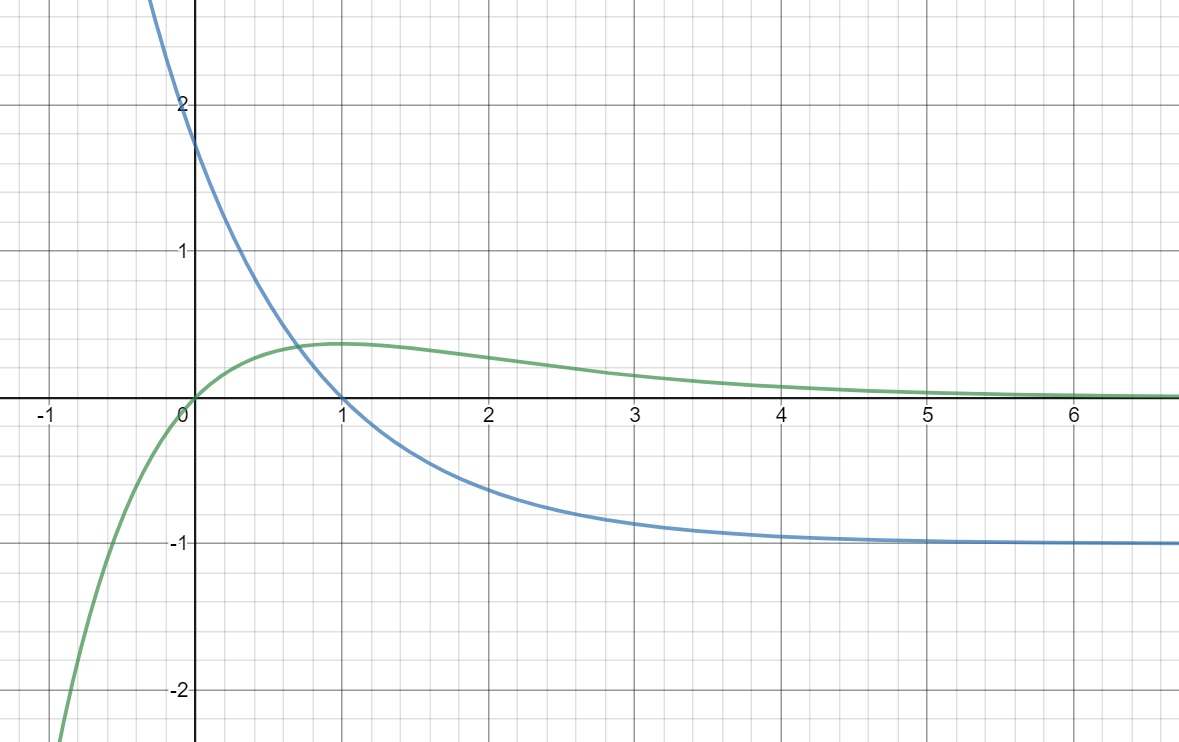
\includegraphics[scale=1]{e1-x-1andxe-x.png}
	\centering
	\caption{$c = -2$, $x_0 = -1$}
\end{figure}
\begin{figure}[!htbp]
	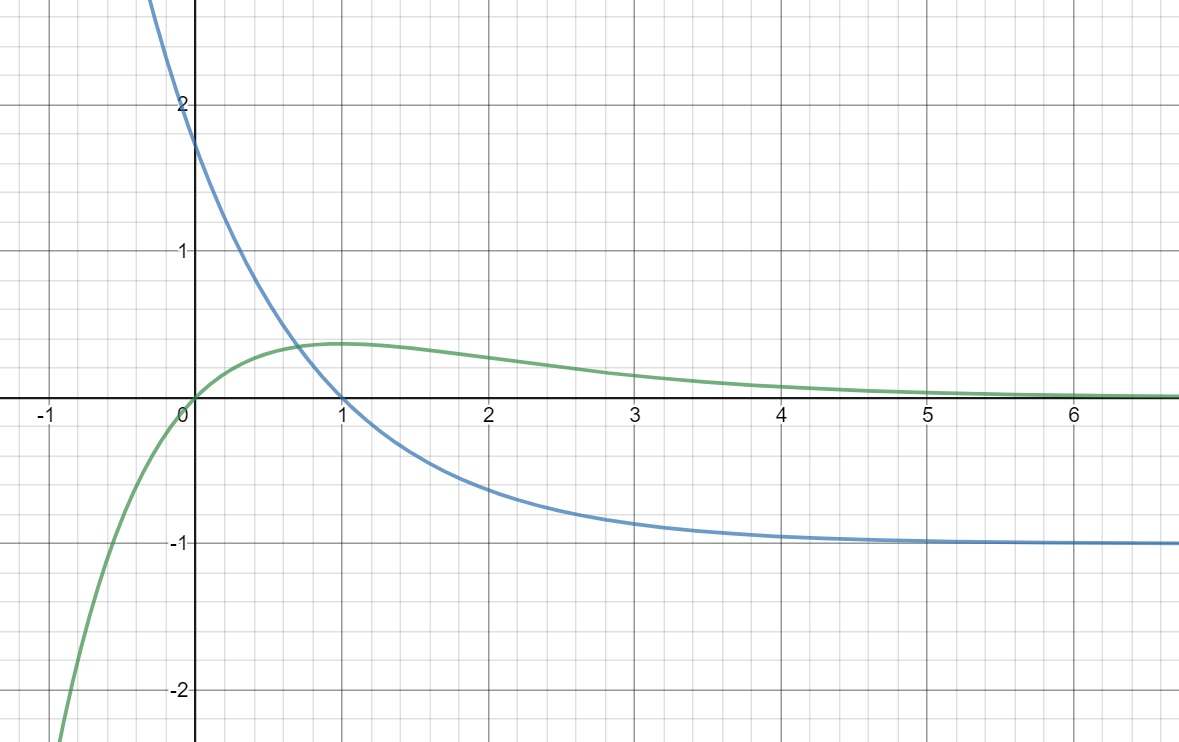
\includegraphics[scale=1]{e1-x-1andxe-x.png}
	\centering
	\caption{$c = -2$, $x_0 = 1.99999999999999$}
\end{figure}
\begin{figure}[!htbp]
	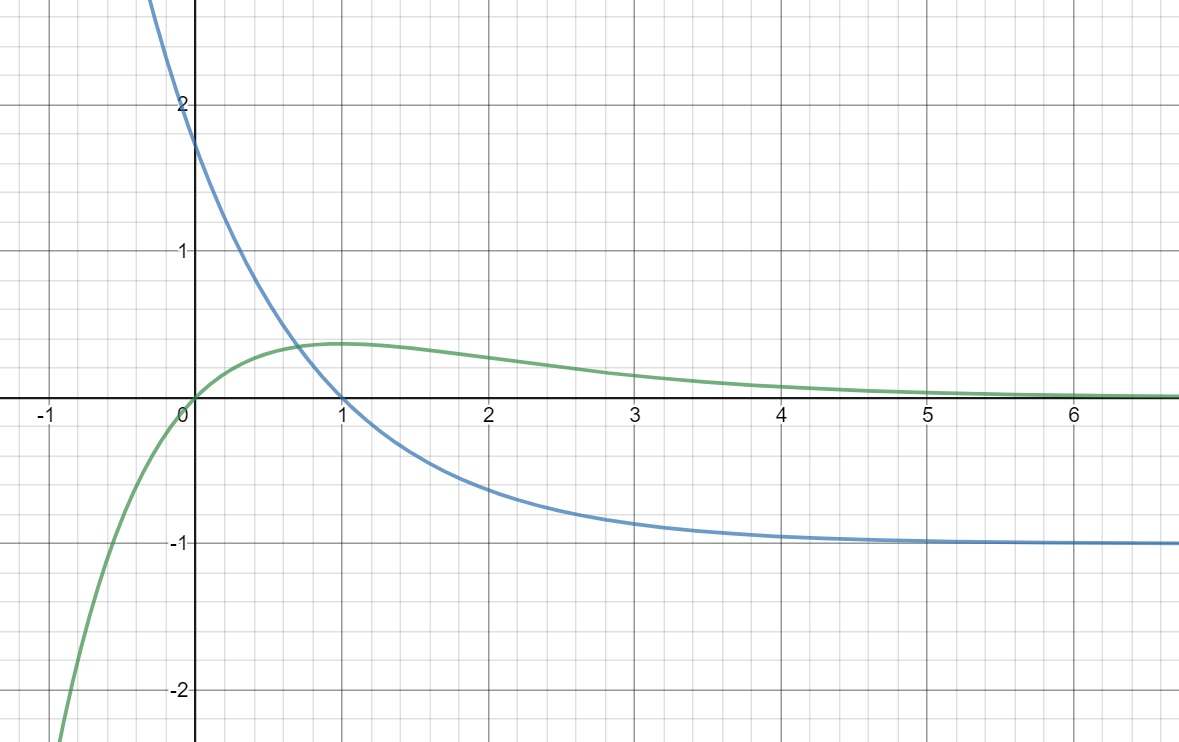
\includegraphics[scale=1]{e1-x-1andxe-x.png}
	\centering
	\caption{$c = -1$, $x_0 = 1$}
\end{figure}



Wnioski. Zauważmy, że w tym zadaniu również mamy do czynienia ze zjawiskiem sprzężenia zwrotnego. W całym zadaniu możemy wyróżnić 3 typy doświadczeń. Pierwszy z nich to dwa pierwsze doświadczenia oraz te z c = -1 i $x_0 \in \{-1,1\}$, w którch otrzymano ciągi stałe lub naprzemienne, są to układy stabilne. Zauważmy też, że punkty $-1$ i $2$ są punktami stałymi funkcji $x^2 - 2$. Właśnie dlatego w dwóch pierwszych doświadczeniach wartości zbiegają do tych wartości. Drugi typ to doświadczenie z $x_0 = 1.99999999999999$. Tutaj ciąg był chaotyczny. Jest to układ niestabilny. Trzeci typ doświadczenia reprezentują dwa ostatnie eksperymenty. W obu z nich układ początkowo był chaotyczny, ale po którymś kroku zaczął się stabilizować. Są to układy stabilne.

	
	\begin{table}[!h]
		\centering
		\label{tab:table1}
		\begin{tabular}{|c|c|c|c|}
			\multicolumn{4}{c}{$c = -2$} \\
			\hline
			numer iteracji & $x_0 = 1$ & $x_0 = 2$ & $x_0 = 1.99999999999999$\\
			\hline
			1 & -1 &	 2 &	 1.99999999999996 \\ \hline
			2 & -1 &	 2 &	 1.9999999999998401 \\ \hline
			3 & -1 &	 2 &	 1.9999999999993605 \\ \hline
			4 & -1 &	 2 &	 1.999999999997442 \\ \hline
			5 & -1 &	 2 &	 1.9999999999897682 \\ \hline
			6 & -1 &	 2 &	 1.9999999999590727 \\ \hline
			7 & -1 &	 2 &	 1.999999999836291 \\ \hline
			8 & -1 &	 2 &	 1.9999999993451638 \\ \hline
			9 & -1 &	 2 &	 1.9999999973806553 \\ \hline
			10 & -1 &	 2 &	 1.999999989522621 \\ \hline
			11 & -1 &	 2 &	 1.9999999580904841 \\ \hline
			12 & -1 &	 2 &	 1.9999998323619383 \\ \hline
			13 & -1 &	 2 &	 1.9999993294477814 \\ \hline
			14 & -1 &	 2 &	 1.9999973177915749 \\ \hline
			15 & -1 &	 2 &	 1.9999892711734937 \\ \hline
			16 & -1 &	 2 &	 1.9999570848090826 \\ \hline
			17 & -1 &	 2 &	 1.999828341078044 \\ \hline
			18 & -1 &	 2 &	 1.9993133937789613 \\ \hline
			19 & -1 &	 2 &	 1.9972540465439481 \\ \hline
			20 & -1 &	 2 &	 1.9890237264361752 \\ \hline
			21 & -1 &	 2 &	 1.9562153843260486 \\ \hline
			22 & -1 &	 2 &	 1.82677862987391 \\ \hline
			23 & -1 &	 2 &	 1.3371201625639997 \\ \hline
			24 & -1 &	 2 &	 -0.21210967086482313 \\ \hline
			25 & -1 &	 2 &	 -1.9550094875256163 \\ \hline
			26 & -1 &	 2 &	 1.822062096315173 \\ \hline
			27 & -1 &	 2 &	 1.319910282828443 \\ \hline
			28 & -1 &	 2 &	 -0.2578368452837396 \\ \hline
			29 & -1 &	 2 &	 -1.9335201612141288 \\ \hline
			30 & -1 &	 2 &	 1.7385002138215109 \\ \hline
			31 & -1 &	 2 &	 1.0223829934574389 \\ \hline
			32 & -1 &	 2 &	 -0.9547330146890065 \\ \hline
			33 & -1 &	 2 &	 -1.0884848706628412 \\ \hline
			34 & -1 &	 2 &	 -0.8152006863380978 \\ \hline
			35 & -1 &	 2 &	 -1.3354478409938944 \\ \hline
			36 & -1 &	 2 &	 -0.21657906398474625 \\ \hline
			37 & -1 &	 2 &	 -1.953093509043491 \\ \hline
			38 & -1 &	 2 &	 1.8145742550678174 \\ \hline
			39 & -1 &	 2 &	 1.2926797271549244 \\ \hline
			40 & -1 &	 2 &	 -0.3289791230026702 \\ \hline
		\end{tabular}
	\end{table}
	
	\begin{table}[!h]
		\centering
		\label{tab:table1}
		\begin{tabular}{|c|c|c|c|c|}
			\multicolumn{5}{c}{$c = -1$} \\
			\hline
			numer iteracji & $x_0 = 1$ & $x_0 = -1$ & $x_0 = 0.25$ & $x_0 = 0.75$ \\
			\hline
			1	&0 &	0 &	-0.4375 &	 -0.9375 \\ \hline	
			2	& -1 &	 -1 &	 -0.80859375 &	 -0.12109375 \\ \hline	
			3	& 0 &	 0 &	 -0.3461761474609375 &	 -0.9853363037109375 \\ \hline	
			4	& -1 &	 -1 &	 -0.8801620749291033 &	 -0.029112368589267135 \\ \hline	
			5	& 0 &	 0 &	 -0.2253147218564956 &	 -0.9991524699951226 \\ \hline	
			6	& -1 &	 -1 &	 -0.9492332761147301 &	 -0.0016943417026455965 \\ \hline	
			7	& 0 &	 0 &	 -0.0989561875164966 &	 -0.9999971292061947 \\ \hline	
			8	& -1 &	 -1 &	 -0.9902076729521999 &	 -5.741579369278327e-6 \\ \hline	
			9	& 0 &	 0 &	 -0.01948876442658909 &	 -0.9999999999670343 \\ \hline	
			10&	 -1 &	 -1 &	 -0.999620188061125 &	 -6.593148249578462e-11 \\ \hline	
			11&	 0 &	 0 &	 -0.0007594796206411569 &	 -1.0 \\ \hline	
			12&	 -1 &	 -1 &	 -0.9999994231907058 &	 0.0 \\ \hline	
			13&	 0 &	 0 &	 -1.1536182557003727e-6 &	 -1.0 \\ \hline	
			14&	 -1 &	 -1 &	 -0.9999999999986692 &	 0.0 \\ \hline	
			15&	 0 &	 0 &	 -2.6616486792363503e-12 &	 -1.0 \\ \hline	
			16&	 -1 &	 -1 &	 -1.0 &	 0.0 \\ \hline	
			17&	 0 &	 0 &	 0.0 &	 -1.0 \\ \hline	
			18&	 -1 &	 -1 &	 -1.0 &	 0.0 \\ \hline	
			19&	 0 &	 0 &	 0.0 &	 -1.0 \\ \hline	
			20&	 -1 &	 -1 &	 -1.0 &	 0.0 \\ \hline	
			21&	 0 &	 0 &	 0.0 &	 -1.0 \\ \hline	
			22&	 -1 &	 -1 &	 -1.0 &	 0.0 \\ \hline	
			23&	 0 &	 0 &	 0.0 &	 -1.0 \\ \hline	
			24&	 -1 &	 -1 &	 -1.0 &	 0.0 \\ \hline	
			25&	 0 &	 0 &	 0.0 &	 -1.0 \\ \hline	
			26&	 -1 &	 -1 &	 -1.0 &	 0.0 \\ \hline	
			27&	 0 &	 0 &	 0.0 &	 -1.0 \\ \hline	
			28&	 -1 &	 -1 &	 -1.0 &	 0.0 \\ \hline	
			29&	 0 &	 0 &	 0.0 &	 -1.0 \\ \hline	
			30&	 -1 &	 -1 &	 -1.0 &	 0.0 \\ \hline	
			31&	 0 &	 0 &	 0.0 &	 -1.0 \\ \hline	
			32&	 -1 &	 -1 &	 -1.0 &	 0.0 \\ \hline	
			33&	 0 &	 0 &	 0.0 &	 -1.0 \\ \hline	
			34&	 -1 &	 -1 &	 -1.0 &	 0.0 \\ \hline	
			35&	 0 &	 0 &	 0.0 &	 -1.0 \\ \hline	
			36&	 -1 &	 -1 &	 -1.0 &	 0.0 \\ \hline	
			37&	 0 &	 0 &	 0.0 &	 -1.0 \\ \hline	
			38&	 -1 &	 -1 &	 -1.0 &	 0.0 \\ \hline	
			39&	 0 &	 0 &	 0.0 &	 -1.0 \\ \hline	
			40&	 -1 &	 -1 &	 -1.0 &	 0.0 \\ \hline	
		\end{tabular}
	\end{table}


\end{document}